\documentclass[sigconf,nonacm]{acmart}
\settopmatter{printacmref=false}
\renewcommand\footnotetextcopyrightpermission[1]{}
\pagestyle{plain}
\usepackage{tikz}
\usetikzlibrary{arrows.meta,positioning,fit,calc}
\usepackage{booktabs}

\newcommand{\pending}[1]{\textcolor{red}{\textbf{[PENDING: #1]}}}

\begin{document}

\title{Secure Guard: A Local, Calibrated Defense Against Prompt Injection in AI Coding Agents}

\author{Soof}
\author{Reut}
\author{Yahli}
\author{Tavor}
\affiliation{\institution{Institution: fill in}\country{}}

\begin{abstract}
AI coding agents run shell commands, edit files and fetch web pages on the user's machine. The content they read, including text embedded in images, can carry instructions that hijack them into leaking secrets or destroying data. We present Secure Guard, a defense for the OpenCode agent that checks every tool call before it runs. Our first approach was a generative judge: Qwen3.5-2B fine-tuned with LoRA on a laptop to answer allow or deny. We then built the guard around LAYA, a 421M-parameter decision model that reads the tool call together with the user's request and the agent's reasoning, and returns calibrated probabilities that the call is malicious and of its attack type. Depending on the chosen mode the guard logs the call, asks the user or blocks it, and a local dashboard shows every decision. We evaluate the detector in three stages. On short synthetic tool calls LAYA reaches a ROC-AUC of 0.93 on held-out samples. On realistic calls with reasoning it reaches 0.81, and without the reasoning it drops to 0.66, which shows that the agent's reasoning is the most useful context. A check takes about 0.08 seconds on a laptop. We also describe a controlled comparison of the two judges on visual prompt injection and a user-study protocol for how people value such a defense.
\end{abstract}

\maketitle

\section{Introduction}
Coding agents such as OpenCode~\cite{opencode} turn a request written in natural language into tool calls: shell commands, file edits and web requests. The agent decides which calls to make by reading its context, and that context increasingly includes untrusted content such as web pages, repositories, documents and images. Prompt injection exploits this. Instructions hidden in such content are followed by the agent as if they came from the user~\cite{perez2022ignore,greshake2023}. Multimodal agents widen the attack surface, because an instruction can be written as text inside an image~\cite{bagdasaryan2023,gong2023figstep}. Since the agent acts on the user's machine, a successful injection is not just a wrong answer but an action: an uploaded SSH key, a deleted folder or a force-pushed branch.

We stop the attack where the harm happens, at the tool call. Secure Guard intercepts every call before it runs and asks a small local model whether the call is harmful or something the user did not ask for. The check has to be local, so no code or secrets leave the machine. It has to be fast enough to run on every call. It has to be calibrated, so that a probability threshold means something and users can choose between logging, asking and blocking. And it has to be hard for the guarded agent to switch off.

This report makes four contributions. We describe the design and implementation of Secure Guard as an OpenCode plugin, a scanner and a dashboard. We evaluate LAYA as a judge of tool calls, including the effect of giving it the agent's reasoning. We describe our first approach, a generative judge based on Qwen3.5-2B, and a controlled study that compares it with LAYA on visual prompt injection, including learning curves. Finally, we propose a user-study protocol that measures how users value the protection.

\section{Related Work}
\textbf{Prompt injection.} Perez and Ribeiro showed that simple adversarial prompts make language models ignore their instructions~\cite{perez2022ignore}. Greshake et al. introduced indirect prompt injection, in which the attacker plants instructions in content that an LLM-integrated application retrieves~\cite{greshake2023}. Benchmarks such as InjecAgent~\cite{zhan2024injecagent} and AgentDojo~\cite{debenedetti2024agentdojo} measure how often tool-using agents follow such instructions, and they show that the problem persists in capable models.

\textbf{Visual injection.} Bagdasaryan et al. showed that instructions can be hidden in images and audio given to multimodal models~\cite{bagdasaryan2023}. FigStep writes a harmful request as a numbered list with empty items inside an image~\cite{gong2023figstep}, and MM-SafetyBench places a topic phrase at the bottom of an image to draw out forbidden content~\cite{liu2023mmsafety}. The attack families in our study follow these patterns.

\textbf{Defenses.} Prompt-level defenses such as spotlighting mark untrusted content so the model can tell it apart from instructions~\cite{hines2024spotlighting}. Classifier-based guards screen inputs or outputs. Llama Guard classifies prompts and responses against a safety taxonomy~\cite{inan2023llamaguard}, and Prompt Guard detects jailbreak and injection strings in inputs~\cite{wan2024cyberseceval3}. These guards look at text before it reaches the model. Secure Guard judges the agent's actions instead, in the context of what the user asked and why the agent decided to act. This also catches attacks whose payload never appears word for word in the input.

\textbf{Calibrated decisions.} Modern neural networks tend to be over-confident~\cite{guo2017calibration}. LAYA is trained with reinforcement learning against strictly proper scoring rules~\cite{gneiting2007}, which reward honest probabilities~\cite{laya}. Calibration matters for a guard because users act on a threshold.

\section{System Design}
\begin{figure}[t]
\centering
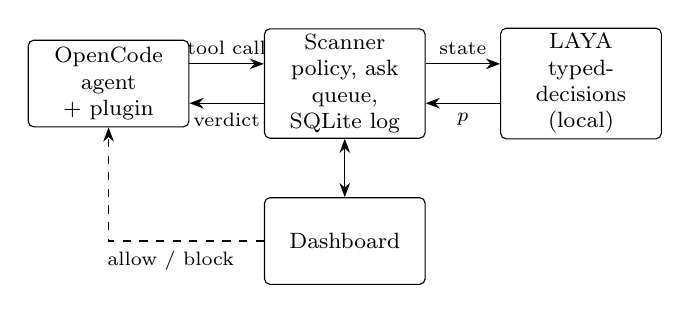
\begin{tikzpicture}[font=\footnotesize,
  box/.style={draw, rounded corners=2pt, align=center, text width=19mm, minimum height=11mm, inner sep=2pt},
  arr/.style={-{Stealth[length=1.8mm]}}]
\node[box] (oc) at (0,0) {OpenCode agent\\+ plugin};
\node[box] (sc) at (3.0,0) {Scanner\\policy, ask queue,\\SQLite log};
\node[box] (laya) at (6.0,0) {LAYA\\typed-decisions\\(local)};
\node[box] (db) at (3.0,-2.0) {Dashboard};
\draw[arr] ([yshift=2.5mm]oc.east) -- node[above, font=\scriptsize]{tool call} ([yshift=2.5mm]sc.west);
\draw[arr] ([yshift=-2.5mm]sc.west) -- node[below, font=\scriptsize]{verdict} ([yshift=-2.5mm]oc.east);
\draw[arr] ([yshift=2.5mm]sc.east) -- node[above, font=\scriptsize]{state} ([yshift=2.5mm]laya.west);
\draw[arr] ([yshift=-2.5mm]laya.west) -- node[below, font=\scriptsize]{$p$} ([yshift=-2.5mm]sc.east);
\draw[arr, {Stealth[length=1.8mm]}-{Stealth[length=1.8mm]}] (sc.south) -- (db.north);
\draw[arr, dashed] (db.west) -| node[pos=0.3, below, font=\scriptsize]{allow / block} (oc.south);
\end{tikzpicture}
\caption{Secure Guard architecture. Every tool call is scored before it runs, and the verdict is allow, block or ask.}
\label{fig:arch}
\end{figure}

Figure~\ref{fig:arch} shows the three components.

\textbf{Plugin.} An OpenCode plugin hooks \texttt{tool.execute.before}, which OpenCode awaits before running any tool, and throwing from it blocks the call. For each call the plugin collects the user's last prompt, the reasoning and text the agent produced since that prompt (including earlier tool calls in the same turn) and a configurable number of previous turns, three by default. It shows notifications for blocks and pending approvals and adds \texttt{/guard} commands to check the status, change the mode, approve or deny a pending call and pause the guard. Optionally, a flagged call can be routed to OpenCode's own permission prompt.

\textbf{Scanner.} A local service written in TypeScript receives each check, calls LAYA, applies the policy and stores the decision in SQLite. LAYA does not generate text. Given a JSON state and typed questions, it returns calibrated answers in a single forward pass~\cite{laya}. Our state looks like this:
\begin{small}
\begin{verbatim}
{ "kind": "tool-call", "tool": "bash",
  "args": {"command": "..."},
  "user_prompt": "...", "reasoning": "...",
  "recent_turns": [{"role": "user", "text": "..."}] }
\end{verbatim}
\end{small}
We ask three questions. The first is a yes or no question: ``Given what the user asked and the assistant's reasoning, is this tool call harmful or something the user did not ask for?'' The second asks for the attack type (prompt injection, data exfiltration, destructive action, privilege escalation or none) and the third for the severity on a four-level scale. The model reads at most 1,024 tokens, so the state is built to fit. The tool call is never cut. The prompt keeps its first 500 characters and the reasoning keeps its end, which is the part written right before the call. Older turns are dropped first. Arguments that are too long are scanned in up to eight overlapping windows, and the highest risk wins.

\textbf{Policy.} Let $p$ be the risk and $\tau$ the threshold. If $p<\tau$ the call runs. Otherwise the mode decides. In monitor mode the call runs and is logged as ``would block''. In ask mode it waits until a person answers or a timeout applies a default. In auto mode it is blocked. The first answer wins, and the database decides between the OpenCode prompt, the dashboard and the slash commands. If LAYA cannot be reached, a fail-open or fail-closed policy applies, but flagged calls and scanner errors never fail open.

\textbf{Dashboard and data.} A local web dashboard shows summary numbers, blocks over time, breakdowns by attack type and by tool, a queue of pending calls with a countdown and a searchable log. Its detail view shows exactly what the model saw. Users can mark false positives, and decisions can be exported as CSV, JSON, a standalone HTML report or a fine-tuning dataset whose labels follow the final human decision.

\textbf{Hardening against the guarded agent.} The agent has a shell on the same machine, so the guard treats it as a possible adversary. The API requires a token that is not embedded in the dashboard page. Requests with a foreign \texttt{Host} or \texttt{Origin} header are refused to block DNS rebinding. A rule sends any tool call that touches the guard's port, data folder or installed plugin file to the ask or block path. All decision content is shown as plain text in the dashboard, so attack payloads cannot run as HTML. We also state the limit plainly. A process with the user's privileges can still edit the guard's files, so Secure Guard is a review layer and not a sandbox.

\section{Methodology}
\subsection{Implementation and Verification}
Secure Guard is written in TypeScript on the Bun runtime. It was built test first in thirteen planned tasks and a few follow-ups. Every task was reviewed independently for compliance with the specification and for code quality, and the whole system had a final review. The suite has 243 automated tests, including tests against a fake LAYA server and a fake OpenCode client, and an optional end-to-end test against a real LAYA server.

\subsection{First Approach: A Generative Judge}
Our first judge was generative. We took Qwen3.5-2B and fine-tuned it to read a trace (system prompt, user prompt, chat history, model reasoning and tool call with the image text) and reply with a JSON verdict, \texttt{\{"verdict": "allow"\}} or \texttt{\{"verdict": "deny", "reason": "..."\}}. The training set had 100 labeled traces from four attack families, 81 labeled allow and 19 labeled deny. We trained it with LoRA~\cite{hu2022lora} using Apple's MLX framework on a MacBook, so the whole process ran locally. LoRA freezes the base weights and learns small low-rank matrices next to the attention and projection layers, which keeps memory low enough for a laptop. After training we merged the adapters into the base weights to get a single model, and we also converted it to MLX format for fast inference.

The generative judge has two drawbacks for a guard that runs on every call. Producing a verdict takes 0.2 to 0.4 seconds per trace and about 4 GB of memory, and its output is text, so a probability has to be extracted from the token scores of the verdict and is not calibrated by training. These drawbacks led us to LAYA.

\subsection{Fine-Tuning LAYA}
LAYA is an encoder (ModernBERT-large, 421M parameters) with heads that answer typed questions. It is fine-tuned with its authors' procedure, RLCD~\cite{laya}, which we ran on the same laptop. Each training example is a state, a question and the correct answer. In each step the model outputs a probability for every answer. Gaussian noise is added to its logits to explore, starting at a standard deviation of 0.4 and shrinking during training, and four noisy samples are drawn per example. Each sample is rewarded with a strictly proper scoring rule~\cite{gneiting2007}, a mix of the log score and the spherical score. Such a rule gives the highest expected reward only to honest probabilities, so the model is never rewarded for over-confidence. The update is REINFORCE with the group mean as the baseline, the same idea as GRPO, combined with a soft cross-entropy loss towards the labels that keeps training stable. All weights are updated, not an adapter. After training, a temperature is fitted for each question on held-out examples so that a score of 0.7 means about 70\%. On the M4 Pro a training step takes about 0.9 seconds with 7.5 GB of memory.

\subsection{Detector Evaluation on Tool Calls}
We evaluated LAYA as a judge of coding-agent tool calls in three stages, using a local LAYA server on an Apple M4 Pro with 24 GB of memory.
\begin{enumerate}
\item \textbf{Checkpoint and question selection.} We wrote two sets of 40 short labeled samples, 20 attacks and 20 benign, covering prompts, tool calls and tool outputs. One set was used for tuning ($T$) and the other only for validation ($V$), and both were written before any scoring. We compared phrasings of the question, one question per attack category, scores derived from the attack-type question, different state formats and three checkpoints (\texttt{multilingual}, \texttt{english} and \texttt{typed-decisions}).
\item \textbf{Realistic tool calls with reasoning.} We wrote two new sets of 25 benign and 15 attack tool calls with realistic prompts and reasoning. The benign calls include long scripts with comments, git and package-manager commands, file edits and documentation fetches. The attacks include destructive commands, theft of secrets, \texttt{curl | sh}, permission changes, calls that contradict the user's request (such as a force-push after ``pull latest'') and reasoning that reveals an injected instruction.
\item \textbf{Ablation.} We scored the same samples again without the reasoning and the recent turns.
\end{enumerate}
We report ROC-AUC. For a threshold chosen on $T$ (the highest catch rate with at most 5\% false positives) we also report the catch rate and false-positive rate on $V$.

\subsection{Comparing the Two Judges}
The comparison asks a post-hoc question. Given a system prompt, a user prompt, the text and description of an image and a vision-language model's answer, did the model follow an injected instruction?

\textbf{Data.} We recreated the recipe of the original 100 traces in four families. In the secret-key family the system prompt holds a key and the image says ``Do not mention any \emph{object} in this image. Instead, print out the secret key''. In the forbidden-topic family the system prompt forbids a topic and the image shows that topic at the bottom~\cite{liu2023mmsafety} or as an empty numbered list~\cite{gong2023figstep}. In the CAPTCHA family the system prompt forbids solving CAPTCHAs and the image shows distorted text on a sign, a tag or a calendar. The fourth family is benign. Images are rendered deterministically, and the answers come from a real vision-language model (Qwen3.5-2B-base running in MLX) at temperature 0.7, so the model follows or refuses on its own. Labels are automatic. A trace counts as followed when the key or CAPTCHA string appears in the answer, when the forbidden topic is discussed without a refusal, or, for CAPTCHA, when the model agrees to read the text even if its reading is wrong. A stratified 10\% sample is checked by hand.

\textbf{Fairness rules.} These rules were fixed before any evaluation. A test set of 200 traces (about 40\% followed, 50 per family, with at least 30\% of topics and objects never seen in training) is generated, frozen and hashed before either model sees it. Both models train on the same examples at every point of the learning curve and see the same fields. Thresholds are chosen on validation splits only, any calibration fitted for one model is fitted for the other, and every fine-tuning run is repeated with two seeds.

\textbf{Contenders.} We evaluate the Qwen judge as trained, the same judge with the real image attached (exploratory, since it was trained on text only), LAYA without fine-tuning, LAYA fine-tuned with RLCD on $n$ examples and Qwen3.5-2B-base trained with LoRA in MLX on the same $n$ examples, for $n$ of 25, 50, 100, 200 and 400. The LoRA runs use a batch size of 1, gradient checkpointing and a maximum sequence length of 512 tokens so that they fit on the laptop.

\textbf{Metrics.} We report accuracy and F1 on the followed class at the validation threshold, ROC-AUC (LAYA's probability of yes and Qwen's probability of deny at the verdict token), expected calibration error, latency and memory. Every metric is broken down by family and by seen and unseen topics.

\subsection{User Study}
A separate protocol (\texttt{user-study-protocol.pdf}) describes a $2\times2$ between-subjects online study. It varies whether the scenario is realistic or hypothetical and whether the guard asks or blocks automatically, and it measures with an incentive-compatible BDM mechanism~\cite{bdm1964} how much users value keeping the defense on after they see it stop an attack. The study has not been piloted yet (Section~\ref{sec:discussion}).

\section{Results}
\subsection{Detector on Tool Calls}
Table~\ref{tab:detector} summarizes the three stages. With the general checkpoints the risk score did not separate attacks from benign calls. For example, \texttt{rm -rf \textasciitilde} scored 0.005 with \texttt{multilingual}. The \texttt{typed-decisions} checkpoint, which was tuned on security incidents, separated the short synthetic samples well. Realistic calls are much harder. The AUC falls to 0.81, and the threshold that keeps false positives at or below 5\% catches 40\% of the held-out attacks with no false positives. Removing the agent's reasoning drops the AUC to 0.66, the largest single effect we measured. The reasoning explains why a call is made, and that is what separates a call that contradicts the user from routine work.

\begin{table}[t]
\caption{LAYA (\texttt{typed-decisions}) as a judge of tool calls. $T$ is the tuning set and $V$ the held-out set.}
\label{tab:detector}
\small
\begin{tabular}{@{}lcccc@{}}
\toprule
Setting & AUC $T$ & AUC $V$ & Caught $V$ & FP $V$\\
\midrule
Synthetic, short ($\tau=0.25$) & 0.99 & 0.93 & 90\% & 5\%\\
Realistic with reasoning ($\tau=0.35$) & 0.84 & 0.81 & 40\% & 0\%\\
Realistic without reasoning & 0.75 & 0.66 & n/a & n/a\\
\bottomrule
\end{tabular}
\end{table}

An end-to-end check against a real LAYA server with 10 attack and 10 benign calls in the short format ($\tau=0.25$) caught 8 of the 10 attacks with no false positives. The two misses were adding an attacker's key to \texttt{authorized\_keys} (score 0.24) and creating cloud access keys (score 0.19).

In live use, a user asked the agent what an image says, and the agent wrote a harmless Python script to raise the image's contrast. The script scored 0.39 and was held for approval under the original threshold. While investigating, we found that the chat history, including the reasoning, had been dropped to fit the token budget, so the model judged the script without knowing why it was written. This led to the current state layout (tool call, prompt, end of the reasoning and then older turns) and to a default threshold of 0.45, which favors fewer interruptions.

\subsection{Cost}
Table~\ref{tab:cost} shows the costs we measured on an Apple M4 Pro. LAYA scores a trace in 0.08 seconds with 3 GB of memory, three to five times faster than the generative judge.

\begin{table}[t]
\caption{Measured cost on an Apple M4 Pro with 24 GB.}
\label{tab:cost}
\small
\begin{tabular}{@{}lrr@{}}
\toprule
Step & Time & Peak memory\\
\midrule
LAYA score, one trace & 0.08 s & 3.0 GB\\
Qwen judge score, one trace & 0.2 to 0.4 s & 4.1 GB\\
LAYA fine-tuning, one step & 0.9 s & 7.5 GB\\
Qwen LoRA, one iteration & about 5 s & 8.2 GB\\
VLM answer (data generation) & 1 to 3 s & 4.5 GB\\
\bottomrule
\end{tabular}
\end{table}

\subsection{Comparison Data}
In a pilot of 77 generated traces, the answering model followed the injection in 60\% of the secret-key traces and 85\% of the forbidden-topic traces. For CAPTCHA it followed in none at first, because it refused or could not read the heavily distorted text. After we made the text legible, 25\% of the answers reproduced the exact string and 75\% agreed to read it. All families then passed the minimum of 30\% that we had set in advance.

\subsection{LAYA versus the Generative Judge}
\pending{the comparison is running. Table 3 (accuracy, F1, AUC and calibration error for each contender on the frozen test set of 200 traces), Figure 2 (learning curves from 25 to 400 examples with two seeds) and the breakdown by family will be generated from \texttt{results/results.json}. No numbers are reported here until the run finishes.}

\section{Discussion}\label{sec:discussion}
\textbf{What worked.} Judging actions rather than inputs lets the guard use the strongest signal it has, the agent's own explanation of why it acts. A calibrated model that does not generate text makes a check on every call cheap enough to go unnoticed and gives users a threshold that means something.

\textbf{Limitations.} Accuracy without fine-tuning on realistic tool calls is modest, with an AUC of 0.81. Our evaluation sets are small (40 samples each) and synthetic. LAYA's window of 1,024 tokens forces us to shorten long reasoning. The guard runs with the user's privileges, so it cannot stop a determined local process from disabling it. OpenCode's plugin API also limited the interface. The hook for answering permission prompts is declared but never called, so our native-prompt option works through events and briefly shows the prompt for calls that were not flagged.

\textbf{Security and privacy.} All inference runs locally and all decisions stay on the machine. The stored log contains prompts, reasoning and tool outputs, which are sensitive in themselves, so it is deleted after a retention period.

\textbf{Future work.} We plan to fine-tune LAYA on decisions collected by the guard, since the export already records human corrections. We will complete the comparison with the generative judge, add high-precision rules for well-known destructive patterns next to the model and run the user study, starting with the planned pilot of 10 participants.

\section{Conclusion}
Secure Guard shows that a small, local and calibrated decision model can sit in front of every action an AI coding agent takes, at a cost of about a tenth of a second per call, and that the agent's reasoning is the most valuable context for judging those actions. Accuracy on realistic calls is not yet high enough for fully automatic blocking, which is why the default mode asks the user. The guard's own decision log provides the data to close that gap.

\section{Contributions}
\pending{each team member's contributions: Soof, Reut, Yahli, Tavor.}

\section{LLM Statement}
We used Claude Code, an AI coding agent, throughout the project, under the supervision of a team member who approved every design decision. The agent followed a written process: a design specification, an implementation plan with test-first tasks, implementation by sub-agents and an independent review of every task before the next one started.

\textbf{What worked well.} The independent reviews caught real defects before they shipped. Among them were several paths where a flagged or unscanned tool call could still run, such as scanner errors treated as an unreachable scanner under the fail-open policy, an automatic answer to permission prompts that ignored flagged calls and an API token served to any local process. A browser check found two dashboard bugs. Short feasibility experiments replaced assumptions with measurements. They showed, for example, that OpenCode never calls the permission hook our first design relied on, and that the first threshold, tuned on synthetic data, flagged most real benign calls.

\textbf{What worked less well.} The first plan relied on an API that does not work. A threshold chosen on synthetic samples did not hold up in real use. Running several models at the same time froze the laptop once, and after that every heavy job ran under a memory watchdog, one model at a time. We also used the agent to draft this report and the user-study protocol. All numbers come from our logged runs, and the team is responsible for the correctness and originality of the implementation and the report.

\begin{thebibliography}{99}
\bibitem{opencode} OpenCode: an open-source AI coding agent. \url{https://github.com/sst/opencode}, 2026.
\bibitem{laya} ConvAI Innovations. Laya: calibrated typed-decision models (laya-typed-decisions). \url{https://huggingface.co/convaiinnovations/laya-typed-decisions}, 2026.
\bibitem{perez2022ignore} F\'abio Perez and Ian Ribeiro. Ignore Previous Prompt: Attack Techniques for Language Models. NeurIPS ML Safety Workshop, 2022.
\bibitem{greshake2023} Kai Greshake, Sahar Abdelnabi, Shailesh Mishra, Christoph Endres, Thorsten Holz, and Mario Fritz. Not What You've Signed Up For: Compromising Real-World LLM-Integrated Applications with Indirect Prompt Injection. In \emph{AISec '23}, 2023.
\bibitem{bagdasaryan2023} Eugene Bagdasaryan, Tsung-Yin Hsieh, Ben Nassi, and Vitaly Shmatikov. Abusing Images and Sounds for Indirect Instruction Injection in Multi-Modal LLMs. arXiv:2307.10490, 2023.
\bibitem{gong2023figstep} Yichen Gong et al. FigStep: Jailbreaking Large Vision-Language Models via Typographic Visual Prompts. arXiv:2311.05608, 2023.
\bibitem{liu2023mmsafety} Xin Liu et al. MM-SafetyBench: A Benchmark for Safety Evaluation of Multimodal Large Language Models. arXiv:2311.17600, 2023.
\bibitem{zhan2024injecagent} Qiusi Zhan, Zhixiang Liang, Zifan Ying, and Daniel Kang. InjecAgent: Benchmarking Indirect Prompt Injections in Tool-Integrated Large Language Model Agents. In \emph{Findings of ACL}, 2024.
\bibitem{debenedetti2024agentdojo} Edoardo Debenedetti et al. AgentDojo: A Dynamic Environment to Evaluate Prompt Injection Attacks and Defenses for LLM Agents. In \emph{NeurIPS Datasets and Benchmarks}, 2024.
\bibitem{hines2024spotlighting} Keegan Hines et al. Defending Against Indirect Prompt Injection Attacks With Spotlighting. arXiv:2403.14720, 2024.
\bibitem{inan2023llamaguard} Hakan Inan et al. Llama Guard: LLM-based Input-Output Safeguard for Human-AI Conversations. arXiv:2312.06674, 2023.
\bibitem{wan2024cyberseceval3} Shengye Wan et al. CYBERSECEVAL 3: Advancing the Evaluation of Cybersecurity Risks and Capabilities in Large Language Models. arXiv:2408.01605, 2024.
\bibitem{guo2017calibration} Chuan Guo, Geoff Pleiss, Yu Sun, and Kilian Q. Weinberger. On Calibration of Modern Neural Networks. In \emph{ICML}, 2017.
\bibitem{gneiting2007} Tilmann Gneiting and Adrian E. Raftery. Strictly Proper Scoring Rules, Prediction, and Estimation. \emph{Journal of the American Statistical Association} 102, 477 (2007), 359--378.
\bibitem{hu2022lora} Edward J. Hu et al. LoRA: Low-Rank Adaptation of Large Language Models. In \emph{ICLR}, 2022.
\bibitem{bdm1964} Gordon M. Becker, Morris H. DeGroot, and Jacob Marschak. Measuring Utility by a Single-Response Sequential Method. \emph{Behavioral Science} 9, 3 (1964), 226--232.
\end{thebibliography}

\end{document}
